%% LaTeX Beamer presentation template (requires beamer package)
%% see http://latex-beamer.sourceforge.net/
%% idea contributed by H. Turgut Uyar
%% template based on a template by Till Tantau
%% this template is still evolving - it might differ in future releases!

% Voyager presentation for Developers Workshop 2006
% Adrian Gschwend

%\documentclass{beamer}
% Handout:
\documentclass[handout]{beamer}

\mode<presentation>
{
  \usetheme{Warsaw}  
  \setbeamercovered{transparent}
}

\usepackage{amsmath,amssymb}
\usepackage[latin1]{inputenc}
\usepackage{times}
\usepackage[T1]{fontenc}

\beamertemplatetransparentcovereddynamic

\logo{
\includegraphics[height=0.5cm]{dws06.png}}

\title[netlabs.org - The Voyager Project]
{netlabs.org - The Voyager Project}

\subtitle
{A Workplace for the 21th Century}

\author[Adrian Gschwend]
{Adrian~Gschwend}

\institute[netlabs.org]
{
  netlabs.org - Open Source Software for OS/2 and eCS
}

\date[8.4.2006]
{DWS 2006, Biel, Switzerland}

\subject{OS/2 and eCS development}
\keywords{OS/2 eCS eComStation}

% \AtBeginSubsection[]
% {
  % \begin{frame}<beamer>
    % \frametitle{Overview}
    % \tableofcontents[part-1]
  % \end{frame}
% }


\begin{document}

\begin{frame}
  \titlepage
\end{frame}

\begin{frame}
  \frametitle{Outline - Voyager}
  \tableofcontents[part=1,hideallsubsections]
\end{frame}

\part{Voyager}
\section{History}
\subsection{The Idea}
\begin{frame}
\frametitle{The Idea}
\begin{itemize}
      \item long process of thinking about the future for several years
      \item first idea with Kernel of MacOS X in Summer 2004
      \item first presentation of that idea at Developers Workshop 2005 in Dresden
      \item reconsideration of this idea because it doesn't solve the main problem: Desktop
      \item new idea with OpenGL based Desktop with well known toolkits, developed at SYSTEMS fair in Munich
      \item talks to various people and first presentation of that idea at Warpstock Europe 2005 in Dresden
    \end{itemize}   
\end{frame}

\subsection{The Goal}
\begin{frame}
\frametitle{The Goal}
	There are many free desktop environments available, like KDE and GNOME. Our focus is different:
	\begin{itemize}
		\item SOM like object model, binary compatible (unlike everything else out there on Unix)
		\item provide a WPS like desktop environment (OS/2 "Feeling")
		\item well integrated applications (drag and drop, CUA, etc)
		\item focus on localization right from the beginning (Unicode/UTF-8)
		\item keep unique ideas like IOProcs and reimplement them
		\item use as much existing code/apps as possible (as long as it makes sense), don't reinvent the wheel
	\end{itemize}
\end{frame}

\subsection{The middle-term Goal}
\begin{frame}
\frametitle{The middle-term Goal}
	Software takes time to grow, usually more than one thinks. So it is important to have a middle-term strategy as well:
	\begin{itemize}
      \item the development of this project should be possible on many platforms, including eCS
      \item in parallel, we should provide support for the most popular Unix-like systems at the moment
      \item eCS developers should be motivated to use SOM for new ideas because code can be reused
      \item users can continue to use eCS as we know it today and still get new features
      \item in middle-term we can start a smooth migration to the new desktop
    \end{itemize}      
\end{frame}


\subsection{The long-term Goal}
\begin{frame}
\frametitle{The long-term Goal}
	While eCS is a platform that works fine nowadays we won't have any more support from IBM for new hardware, so in long-term we need something else:
	\begin{itemize}
      \item a team of interested developers might start working on an OS/2 compatibility layer for Unix like systems
      \item in long term we need a new kernel, that discussion is absolutely open right now
      \item most of the OS/2 coders don't like the Linux Design so other options are preferred
      \item if you can help out on that project, you are very welcome :)
      \item final goal: our own distribution based on existing and new software
      \item and finally: world domination (aka \it{Stage 3})
    \end{itemize}
\end{frame}

\section{The Voyager Project}
\subsection{Voyager Components}
\begin{frame}
\frametitle{Voyager Components}
	\begin{itemize}
		\item Voyager Object Model
		\item Window Manager (for Cairo and Xlib)
		\item Cairo as GPI replacement (opinions?)
		\item OpenGL based Cairo backend
		\item Xorg OpenGL device drivers (no Xlib necessary in mid-term)
		\item Xlib - see Everblue presentation
		\item open question: Input Handling - who can help?
		\item anything missing? 
	\end{itemize}
\end{frame}

\subsection{Voyager Object Model}
\begin{frame}
\frametitle{Voyager Object Model}
	\begin{itemize}
		\item SOM is a binary compatible object model, no need to recompile objects (unlike on GNOME for example)
		\item there are some design documents from IBM itself (published in ACM)
		\item there is quite some documentation available written by former IBM employees
		\item Chris Wohlgemuth started to reimplement SOM from scratch, see Voyager Object Model presentation
		\item drawback: not many people know SOM - but we are used to that fact as OS/2 users ;-)
	\end{itemize}
\end{frame}

\subsection{Cairo}
\begin{frame}
\frametitle{Cairo}
	\begin{itemize}
		\item modern, open source, cross-platform 2D API
		\item PDF/PS-like 2D API (hint: MacOS X Quartz)
		\item multiple output systems (screen, printer)
		\item OS/2 port exists, not accelerated so far
		\item OpenGL based backend exists, called Glitz (hint: MacOS X Quartz :)
	\end{itemize}
\end{frame}

\subsection{Voyager Security}
\begin{frame}
\frametitle{Voyager Security}
	Most desktops nowadays do have security problems, we try to do it better:
	\begin{itemize}
      \item each developer should think about the consequences of his code in terms of security
      \item peer-reviews of sourcecode by other developers
      \item there are many papers available regarding security, many are already linked in the Voyager wiki
      \item a binary object model doesn't make it easier, Apple had to learn that as well
      \item use existing research work know how (like DOpE - http://os.inf.tu-dresden.de/dope/)
	\end{itemize}
\end{frame}


\subsection{Toolkit}
\begin{frame}
\frametitle{Toolkit}
	\begin{itemize}
		\item modern toolkits are much simpler to use than PM
		\item GTK+ or qt are the options for existing ones, main toolkit will be GTK+
			\begin{itemize}
				\item GTK+ is C, wrappers for all kind of languages
				\begin{itemize}
					\item SWT for GTK+
					\item wxWidgets on top of GTK+
					\item Firefox \& Thunderbird are using GTK+
				\end{itemize}
				\item qt is C++ only, one should support it
			\end{itemize}
		\item We don't need yet another toolkit \texttrademark 
	\end{itemize}
\end{frame}

\subsection{Window Manager}
\begin{frame}
\frametitle{Window Manager}
	\begin{itemize}
      \item the open client windows
      \item the client stacking order
      \item the client to virtual desktop assignment
      \item the session
      \item multiple screens
      \item client decorations
      \item ...
	\end{itemize}
\end{frame}

\subsection{IOProc Replacement}
\begin{frame}
\frametitle{IOProc Replacement}
	The OS/2 way to abstract codecs and such stuff is quite unique
	\begin{itemize}
		\item see \it{IOProc Replacement} presentation
	\end{itemize}
\end{frame}

\section{OpenGL Backend}

\subsection{Motivation}
\begin{frame}
\frametitle{Motivation}
	\begin{itemize}
      \item OpenGL is the standard nowadays, only MS is doing their own game mit DirectX
      \item OpenGL allows fancy stuff like blending and 3D effects, no fun on 2D Hardware
      \item powerful API
      \item MacOS X is using it as backend, Xorg Project is moving towards OpenGL as well
	\end{itemize}
\end{frame}

\subsection{Options Today}
\begin{frame}
\frametitle{Options Today}
	\begin{itemize}
      \item DirectX based Device Drivers - proprietary, binary only and not OpenGL
      \item Xorg device driver backend, open source and used on most Unix platforms, supports OpenGL for new cards (ATI and Nvidia)
      \item SNAP does not have OpenGL and we don't see that changing in the near future
    \end{itemize}
    Our choice should be Xorg Device Driver backend
\end{frame}

\subsection{Xorg OpenGL Design}
\begin{frame}
\frametitle{Xorg OpenGL Design}
	\begin{columns}
		\column[T]{5cm}
			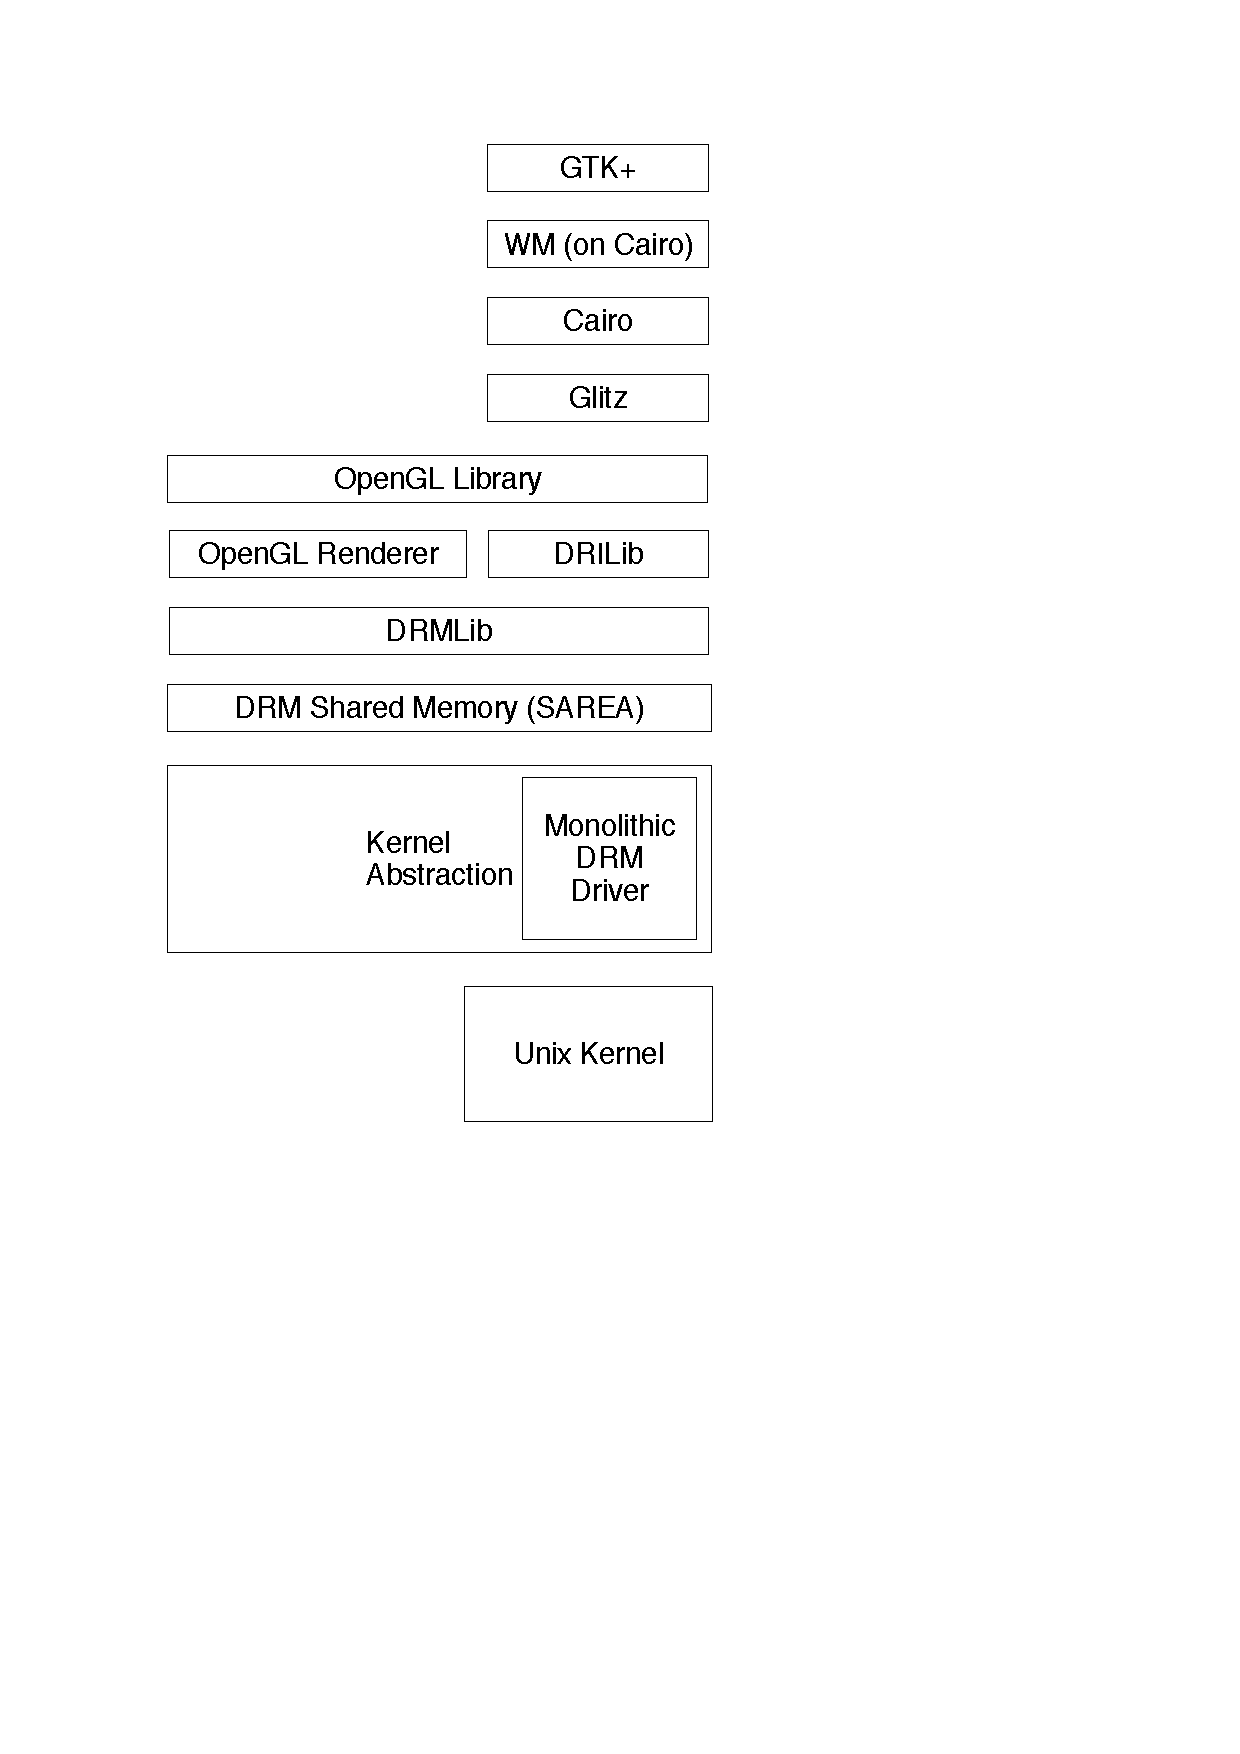
\includegraphics[width=3cm]{ogl-backend.pdf}
		\column{5cm}
		 	Simplified design of the Xorg OpenGL backend (taken from official docs), Xlib stripped out
	\end{columns}
\end{frame}

\section{OS/2 and eCS Compatiblity}
\subsection{Some Ideas}
\begin{frame}
\frametitle{Some Ideas}
	People do ask for binary compatibility. We see the following option:
	\begin{itemize}
      \item use a pure VM based solution - easy and will work well, already possible
      \item rewrite the whole OS as proposed by some people - unrealistic, waste of ressources
      \item implement a minimal OS/2 personality on top of an existing kernel and get binary compatibility to work
	\end{itemize}
\end{frame}

\subsection{OS/2 OS Personality}
\begin{frame}
\frametitle{OS/2 OS Personality}
	To get a minimal OS/2 personality to work we would have to implement:
	\begin{itemize}
      \item DOS*, MOU*, KBD* and VIO* API's
      \item LX loader
      \item GRADD driver for OpenGL backend
      \item what is missing?
    \end{itemize}
	Some things exist, like JdeBP - unfortunately not open source
\end{frame}

\subsection{GRADD on OpenGL}
\begin{frame}
\frametitle{GRADD on OpenGL}
	\begin{columns}
    		\column{3cm}
			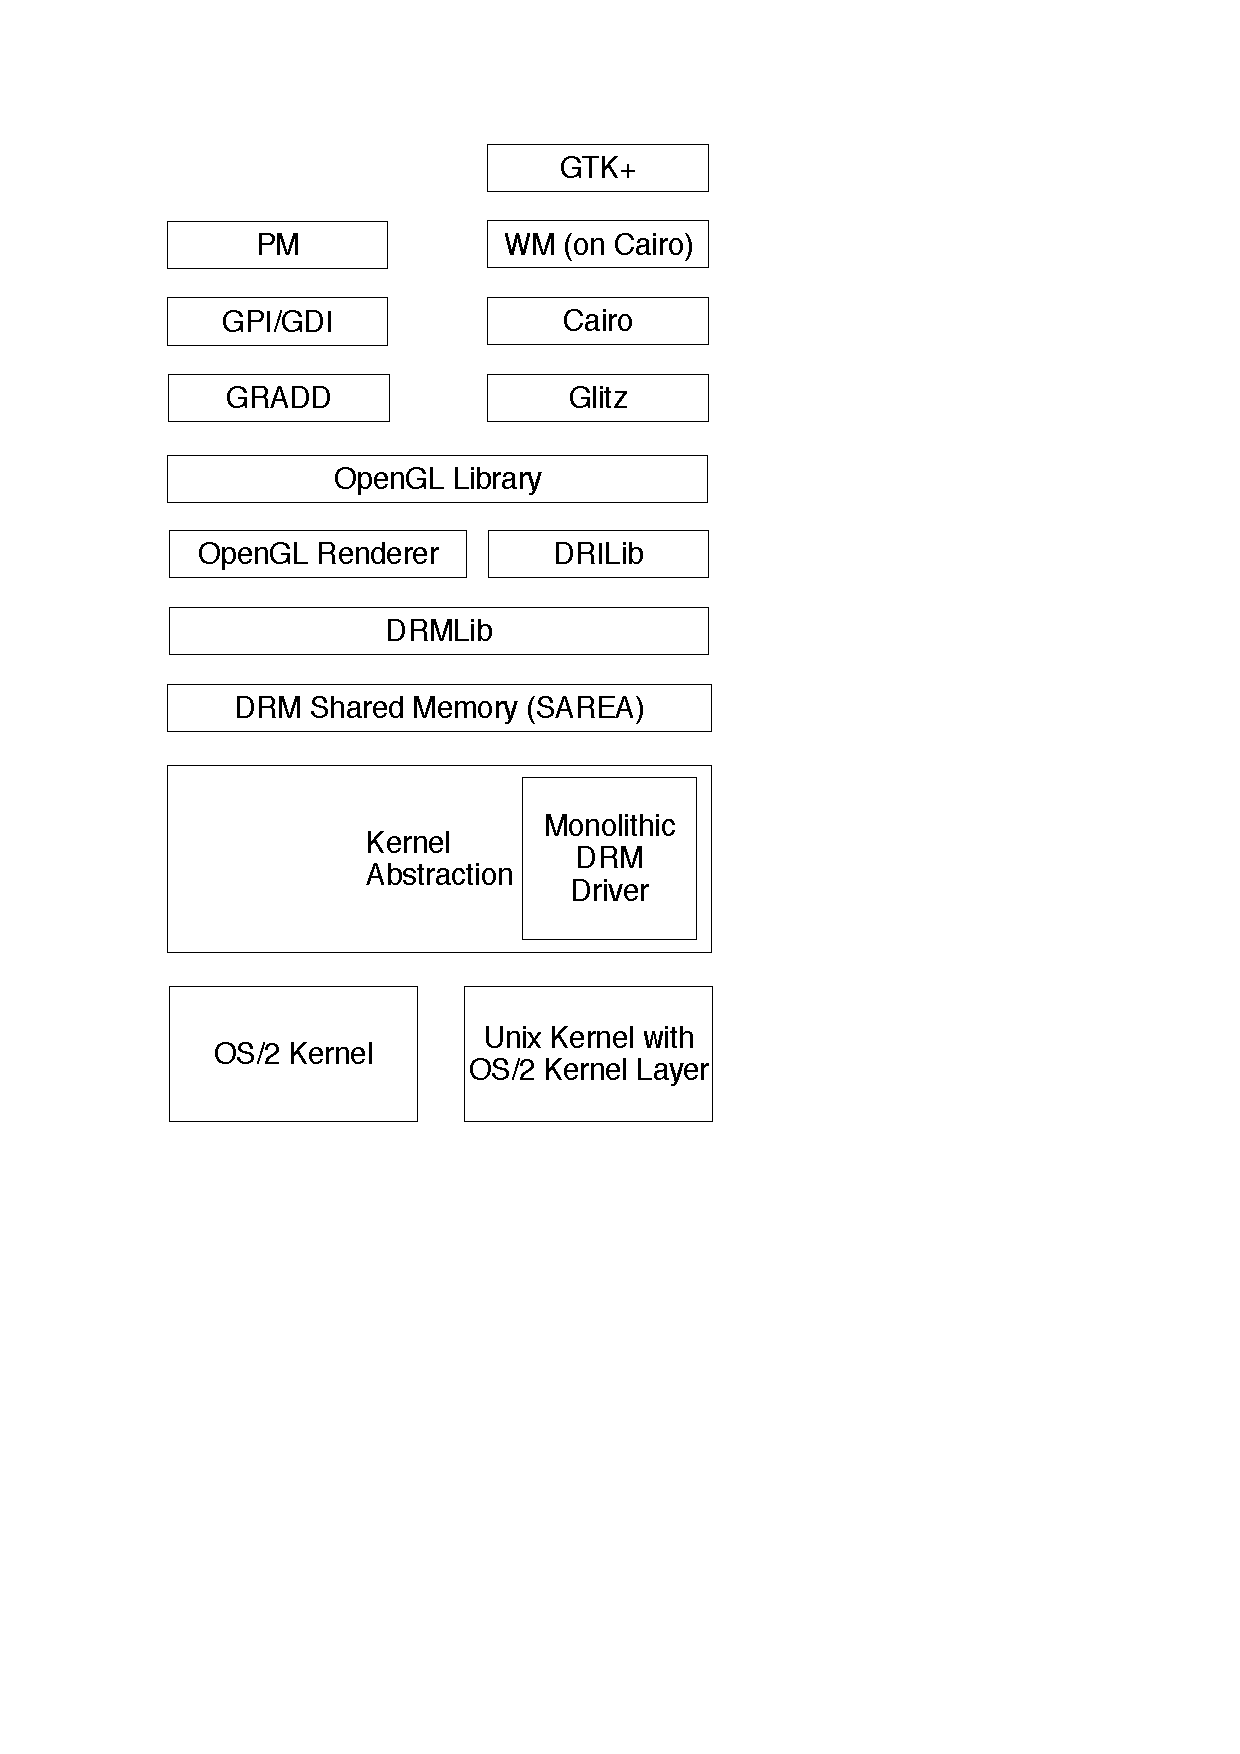
\includegraphics[scale=0.3]{ogl-gradd.pdf}
		\column{6cm}
			\begin{itemize}
              \item OpenGL GRADD driver could be  used on OS/2 already, Xorg should work (with some effort)
              \item As soon as a OS/2 personality would work, one could migrate to the new kernel
            \end{itemize}
  	\end{columns}
\end{frame}



\section{Project Management}
\subsection{Documentation}
\begin{frame}
\frametitle{Documentation}
	Many developers complain about the quality of documentation of some open source projects
	\begin{itemize}
		\item Apple provides very good API docs \& tutorials for Darwin
		\item we must provide that as well, right from the beginning
		\item it should be very easy for new people to get an overview of the projects
		\item see How to organize netlabs.org Software Projects presentation
	\end{itemize}
\end{frame}

\subsection{Coding Guidelines}
\begin{frame}
\frametitle{Coding Guidelines}
	\begin{itemize}
		\item CUA, see http://en.wikipedia.org/wiki/Common\_User\_Access
		\item consistent class \& method names (see Darwin Kernel Programming Guide)
		\item Subversion for sourcecode management
		\item TRAC for milestones, bugs, ToDos, source browsing
		\item see http://svn.netlabs.org/libc as an example
		\item goal: make it easy for new developers to join the projects
	\end{itemize}
\end{frame}

\subsection{License}
\begin{frame}
\frametitle{License}
	\begin{itemize}
		\item we do not want to use (L)GPL for our own code, APL or MPL are candidates
		\item the object model allows binary code, GPL would make that difficult
		\item we might use (L)GPLed code for parts when it makes sense to do that
		\item goal: make the project attractive for commercial vendors right from the beginning
	\end{itemize}
\end{frame}

\section{What's Next?}
\subsection{Next Steps}
\begin{frame}
\frametitle{Next Steps}
	We try to attract developers at this stage already:
	\begin{itemize}
		\item build environment on OS/2
		\item GTK+ for OS/2 (via Everblue)
		\item build environment on Linux
		\item more? FreeBSD, MacOS X, Solaris etc volunteers needed :)
		\item mailinglist for discussions
		\item The Design of Voyager - online design document
	\end{itemize}
	http://wiki.netlabs.org/index.php/Voyager has more information!
\end{frame}

\subsection{Timeline}
\begin{frame}
\frametitle{Timeline}
\begin{itemize}
  \item first sourcecode online in a few weeks (hopefully)
  \item first version of the design document to be released before Q3/06
  \item new server for netlabs.org, new CMS with dedicated Voyager pages (work in progress)
  \item goal: provide development environments for at least two platforms before end of 2006
\end{itemize}
\end{frame}

\subsection{Join the Project}
\begin{frame}
\frametitle{Join the Project}
\begin{itemize}
  \item check the Voyager Wiki & FAQ, monitor netlabs.org pages
  \item join the Voyager Mailinglist at 
  \item join the #netlabs IRC channel (see http://www.ecomstation.com/chat.phtml)
\end{itemize}
\end{frame}

\end{document}